% ======================================================================
%  Windows Credential Reuse: Pass-the-Hash and Pass-the-Key
%  Security Protocols -- course essay (MSc)
%
%  Build: pdflatex main && biber main && pdflatex main && pdflatex main
%  Toolchain: pdfLaTeX + Biber. No shell-escape required.
%
%  Style: minimal article class, Palatino-like serif, numeric citations.
%  Chosen over heavyweight report templates because the deliverable is a
%  ~22 page essay with hand-authored TikZ diagrams, not a thesis.
%  Preamble adapted in spirit from muktapalshikar/getwriting (article class
%  + a curated package set), reimplemented here to avoid vendored fonts.
% ======================================================================
\documentclass[11pt,a4paper]{article}

% ---------- fonts & encoding ----------
\usepackage[T1]{fontenc}
\usepackage[utf8]{inputenc}
\usepackage{mathpazo}          % Palatino clone, safe under pdfLaTeX
\usepackage{microtype}

% ---------- layout ----------
\usepackage[a4paper,margin=2.6cm,headheight=14pt]{geometry}
\usepackage{parskip}
\setlength{\parskip}{0.5em}
\setlength{\emergencystretch}{2em}

% ---------- structure ----------
\usepackage{titlesec}
\titleformat{\section}{\normalfont\large\bfseries}{\thesection}{0.8em}{}
\titlespacing*{\section}{0pt}{1.6em}{0.6em}
\titleformat{\subsection}{\normalfont\normalsize\bfseries}{\thesubsection}{0.7em}{}
\titlespacing*{\subsection}{0pt}{1.2em}{0.4em}

% ---------- floats, tables, figures ----------
\usepackage{graphicx}
\usepackage{booktabs}
\usepackage{array}
\usepackage{tabularx}
\usepackage{subcaption}
\usepackage{float}
\newcolumntype{L}[1]{>{\raggedright\arraybackslash}p{#1}}
\newcolumntype{Y}{>{\raggedright\arraybackslash}X}
\usepackage{enumitem}
\setlist{itemsep=2pt,topsep=3pt}
\graphicspath{{figures/}}

% ---------- colour, diagrams ----------
\usepackage{xcolor}
\definecolor{inkgrey}{RGB}{60,60,60}
\definecolor{termbg}{RGB}{250,250,250}
\usepackage{tikz}
\usetikzlibrary{arrows.meta,positioning,shapes.geometric,fit,backgrounds,calc}
% \usepackage{pgfplots}   % enable only if a chart (not a diagram) is needed

% ---------- terminal / command output ----------
% Used instead of minted to keep the build free of -shell-escape.
\usepackage{listings}
\lstdefinestyle{term}{
  basicstyle=\ttfamily\footnotesize,
  backgroundcolor=\color{termbg},
  frame=single,
  rulecolor=\color{black!15},
  breaklines=true,
  columns=fullflexible,
  keepspaces=true,
  showstringspaces=false,
  xleftmargin=1.2em,
  framexleftmargin=0.6em,
  aboveskip=0.8em,
  belowskip=0.8em
}
\lstset{style=term}

% ---------- quotations & links ----------
\usepackage{csquotes}
\usepackage[colorlinks=true,linkcolor=inkgrey,citecolor=inkgrey,urlcolor=inkgrey]{hyperref}

% ---------- bibliography ----------
\usepackage[backend=biber,style=numeric-comp,sorting=nyt,maxbibnames=6]{biblatex}
\addbibresource{refs.bib}

% ---------- title ----------
\title{\bfseries Windows Credential Reuse:\\[0.3em]
       Pass-the-Hash and Pass-the-Key\\[0.15em]
       against NTLM and Kerberos}
\author{Author One \and Author Two\\[0.4em]
        \small Security Protocols --- MSc}
\date{\today}

\begin{document}
\maketitle

\begin{flushleft}
\small\textbf{PoC repository:} \url{https://github.com/Sirbu-Boeti-Eduard/pass-the-hash-windows}
\end{flushleft}

% ======================================================================
% ABSTRACT
% Position: the same three sentences the article exists to prove, plus what
% the lab showed. No "this paper explores". Write last.
% ======================================================================
\begin{abstract}
% WANT: Windows authenticates against key material, not passwords. NTLM and
% RC4 Kerberos both complete authentication locally from the NT hash, so
% holding the hash is holding the account - no cracking, no replay, no
% protocol break. Lab result: same 16 bytes -> SMB and WinRM session + a TGT.
% Then one line on the control that actually removes the path, one on detection.
%
% \textbf{Keywords:} NTLM, Kerberos, pass-the-hash, lateral movement,
% Active Directory, detection
\end{abstract}

% ======================================================================
% 1. INTRODUCTION  (budget: 1.5 pages)
% Goal: the reader accepts that "password" is the wrong unit of analysis
% before chapter 2 starts defining terms.
% ======================================================================
\section{Introduction}
\label{sec:intro}

\subsection{Motivation}
% TODO
% - Authentication protocols are usually attacked at their design assumptions,
%   not their ciphers. NTLM is a case study: no cryptographic break exists,
%   and yet the protocol is trivially defeated when the wrong secret leaks.
% - Scale of exposure: NTLM is still negotiable across SMB, RPC, WinRM, LDAP,
%   MSSQL and HTTP/Negotiate; AD domain controllers still accept RC4 tickets.
% - Microsoft has announced NTLM's deprecation -- use this as the framing hook:
%   the technique matters most precisely while the protocol is still in place.

\subsection{Problem statement}
% TODO: the single sentence the essay defends. Suggested:
% "Because both protocols allow a client to complete authentication using a
%  locally stored derived key, any disclosure of that key is equivalent to
%  disclosure of the account, regardless of password strength."

\subsection{Contributions}
% TODO: numbered list, 4 items
%   1. A from-first-principles account of the key material Windows holds.
%   2. A derivation-level explanation of why PtH is not replay.
%   3. A reproducible PoC (PtH over SMB/WinRM, PtK to TGT) with captured evidence.
%   4. Measured before/after of the defences that actually stop it.
% Link the repository here (also in the title block).

\subsection{Scope and non-goals}
% TODO: one short paragraph. State that ticket and certificate abuse share the
% same root cause but are out of scope, and say why (different lab requirements).
% Keep this brief: one or two sentences, no defensive justification.

% ======================================================================
% 2. BACKGROUND
% Job: the minimum systems theory a pentester needs to reason about the
% attack and to defend every claim in it. Order matters:
% orientation -> identity -> secret -> derivation -> protocol -> carrier
% -> what is left behind.
% ======================================================================
\section{Background: How Windows Authenticates}
\label{sec:background}

Three things have to line up before any of this makes sense: a secret, a protocol that accepts it,
and a service that will take the protocol's word for it.

Two values sit in an account record and they are not interchangeable. The \textbf{NT hash} is MD4
over the UTF-16LE password: sixteen bytes, no salt, no iteration count, and identical on every
machine for the same password. The \textbf{LM hash} is the older construction, the password
uppercased, cut to fourteen characters, split into two seven-byte halves and used as DES keys. It
is absent by default on current systems and gives you nothing the NT hash does not. When this
article says ``the hash'', it means the NT hash.

Two protocols consume it. \textbf{NTLM} is challenge-response: the server sends a challenge, the
client computes a response from the hash, the server checks that response against its own copy.
\textbf{Kerberos} is ticket-based: the client asks a KDC, which on a domain is a domain
controller, for a ticket, and under RC4-HMAC the key it proves possession with is the NT hash
itself. Neither puts the hash on the wire. A captured exchange is something to crack offline, not
something to log in with.

A hash or a ticket is worth only what accepts it, and Windows spreads that acceptance over a set of
services rather than one remote-access protocol. Table~\ref{tab:services} lists the ones an
engagement meets, what each is for, and what a valid logon buys there.

Each of these borrows the same authentication layer, which is why one hash reaches all of them and
why blocking a port moves the path rather than closing it.

\begin{table}[htbp]
\centering
\small
\renewcommand{\arraystretch}{1.25}
\caption{Services, and what a valid logon buys on each.}
\label{tab:services}
\begin{tabularx}{\textwidth}{@{}>{\raggedright\arraybackslash}m{2.2cm}>{\raggedright\arraybackslash}m{2.6cm}>{\raggedright\arraybackslash}m{4.2cm}Y@{}}
\toprule
Service & Port & What it is for & A valid logon buys \\
\midrule
\rowcolor{gray!7} SMB & 445 & files and printers & share access, and execution via the service control manager \\
\addlinespace[3pt]
\rowcolor{white} MSRPC & 135 + dynamic & remote procedure calls & service creation, scheduled tasks, DCOM \\
\addlinespace[3pt]
\rowcolor{gray!7} WMI & over MSRPC & system management & process creation, queries \\
\addlinespace[3pt]
\rowcolor{white} WinRM & 5985, 5986 & management over HTTP & command execution without a share \\
\addlinespace[3pt]
\rowcolor{gray!7} RDP & 3389 & an interactive desktop & a desktop session \\
\addlinespace[3pt]
\rowcolor{white} LDAP & 389, 636 & directory queries & reads, and the writes its ACL allows \\
\addlinespace[3pt]
\rowcolor{gray!7} MSSQL & 1433 & a database & queries; \texttt{xp\_cmdshell} with sysadmin \\
\bottomrule
\end{tabularx}
\end{table}

NetBIOS is the layer people misplace. It is a session and naming interface from the LAN Manager
era, not an authentication protocol: SMB once rode on it over TCP 139, and modern SMB runs
directly on 445. What survives is the name service, which is why NBT-NS spoofing still works on
networks that have moved on everywhere else, and why LLMNR, the protocol that took the same job
over, deserves the same treatment.

\subsection{Accounts, SIDs, and the access token}
\label{sec:accounts}

Windows keeps two account databases, and they store the same kind of record. The SAM hive on every
workstation and member server holds the local accounts; \texttt{NTDS.dit} on a domain controller
holds the domain's. Both key an account by a security identifier, a domain or machine SID followed
by a relative identifier, and both keep the account's NT hash beside it
(Figure~\ref{fig:two-stores}). The name is only how people refer to the account. The SID is what
every access check, ACL entry and log line uses, which is why renaming an account changes nothing
and recreating one produces a different identity.

% Figure: one account record, held in the SAM hive or in NTDS.dit.
% Used in section 2.1. Values are illustrative, not taken from a real host.
% Two complete cards, not two columns of one table: each store shows only the
% fields it keeps. The grey band crosses both cards and the gap because the
% rows it covers are the fields both stores hold, at the same height.
\begin{figure}[H]
\centering
\footnotesize
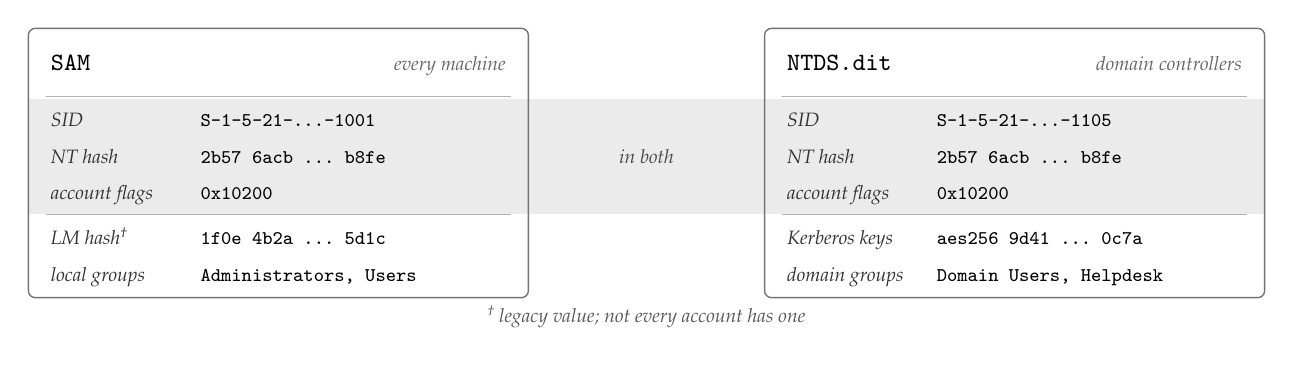
\begin{tikzpicture}[x=1cm,y=1cm,
  card/.style={draw=black!55, line width=0.5pt, rounded corners=2.5pt},
  head/.style={font=\small\ttfamily\bfseries, anchor=base west, inner sep=0pt},
  scope/.style={font=\scriptsize\itshape, text=black!60, anchor=base east,
                inner sep=0pt},
  field/.style={font=\scriptsize\itshape, text=black!80, anchor=base west,
                inner sep=0pt},
  val/.style={font=\scriptsize\ttfamily, anchor=base west, inner sep=0pt}
]

% the shared fields: one band, drawn first so it runs behind both cards
\fill[black!8] (0,-0.90) rectangle (15.7,-2.36);

% the two cards
\draw[card] (0,0) rectangle (6.35,-3.42);
\draw[card] (9.35,0) rectangle (15.7,-3.42);

% header rules and the rule that closes the shared block
\draw[black!30, line width=0.4pt] (0.22,-0.86) -- (6.13,-0.86);
\draw[black!30, line width=0.4pt] (9.57,-0.86) -- (15.48,-0.86);
\draw[black!30, line width=0.4pt] (0.22,-2.36) -- (6.13,-2.36);
\draw[black!30, line width=0.4pt] (9.57,-2.36) -- (15.48,-2.36);

% card headings: store, and the scope it covers
\node[head]  at (0.28,-0.53) {SAM};
\node[scope] at (6.07,-0.53) {every machine};
\node[head]  at (9.63,-0.53) {NTDS.dit};
\node[scope] at (15.42,-0.53) {domain controllers};

% the band's label sits in the gap, on the band itself
\node[font=\scriptsize\itshape, text=black!70, anchor=base]
  at (7.85,-1.71) {in both};

% ---- left card: local account, SAM hive ------------------------------
\node[field] at (0.28,-1.25) {SID};
\node[val]   at (2.18,-1.25) {S-1-5-21-\dots-1001};
\node[field] at (0.28,-1.71) {NT hash};
\node[val]   at (2.18,-1.71) {2b57 6acb \dots\ b8fe};
\node[field] at (0.28,-2.17) {account flags};
\node[val]   at (2.18,-2.17) {0x10200};

\node[field] at (0.28,-2.75) {LM hash\smash{\textsuperscript{\dag}}};
\node[val]   at (2.18,-2.75) {1f0e 4b2a \dots\ 5d1c};
\node[field] at (0.28,-3.21) {local groups};
\node[val]   at (2.18,-3.21) {Administrators, Users};

% ---- right card: domain account, NTDS.dit ----------------------------
\node[field] at (9.63,-1.25) {SID};
\node[val]   at (11.53,-1.25) {S-1-5-21-\dots-1105};
\node[field] at (9.63,-1.71) {NT hash};
\node[val]   at (11.53,-1.71) {2b57 6acb \dots\ b8fe};
\node[field] at (9.63,-2.17) {account flags};
\node[val]   at (11.53,-2.17) {0x10200};

\node[field] at (9.63,-2.75) {Kerberos keys};
\node[val]   at (11.53,-2.75) {aes256 9d41 \dots\ 0c7a};
\node[field] at (9.63,-3.21) {domain groups};
\node[val]   at (11.53,-3.21) {Domain Users, Helpdesk};

% honesty about the legacy value, without cluttering either card
\node[font=\scriptsize\itshape, text=black!65, anchor=base]
  at (7.85,-3.74)
  {\textsuperscript{\dag}\,legacy value; not every account has one};

\end{tikzpicture}
\caption{One account record, two homes.}
\label{fig:two-stores}
\end{figure}


A handful of relative identifiers are fixed, and worth recognising on sight:

\begin{itemize}[leftmargin=1.6em]
  \item \textbf{500} --- the built-in Administrator, on a workstation and on a domain alike.
  \item \textbf{501} --- Guest.
  \item \textbf{502} --- krbtgt, the account whose key encrypts every ticket-granting ticket.
  \item \textbf{512} --- Domain Admins.
  \item \textbf{513} --- Domain Users.
  \item \textbf{515} --- Domain Computers.
\end{itemize}

Everything else starts at 1000 and is issued in order, so the RID of a service account tells you
roughly when it was created.

The logon itself is run by LSASS. \texttt{lsass.exe} is a user-mode process, and the LSA is the
subsystem inside it rather than a second process. The subsystem holds the policy engine, the audit
trail and the table of logon sessions, and builds a token when authentication succeeds. It also
loads the LSA-side instance of each authentication package as a DLL, \texttt{msv1\_0} for NTLM and
the Kerberos package among them, together with the code that reads SAM and the SECURITY hive
(Figure~\ref{fig:lsa-stack}). Callers reach those packages through SSPI, which presents the same
interface to \texttt{winlogon.exe}, to a service, and to your shell.

% Figure: who authenticates, and who authorises. Used in section 2.1.
% Colour carries meaning: blue = process, teal = LSA subsystem, orange =
% authentication package, grey = kernel component. Keep it that way.
\begin{figure}[htbp]
\centering
\small
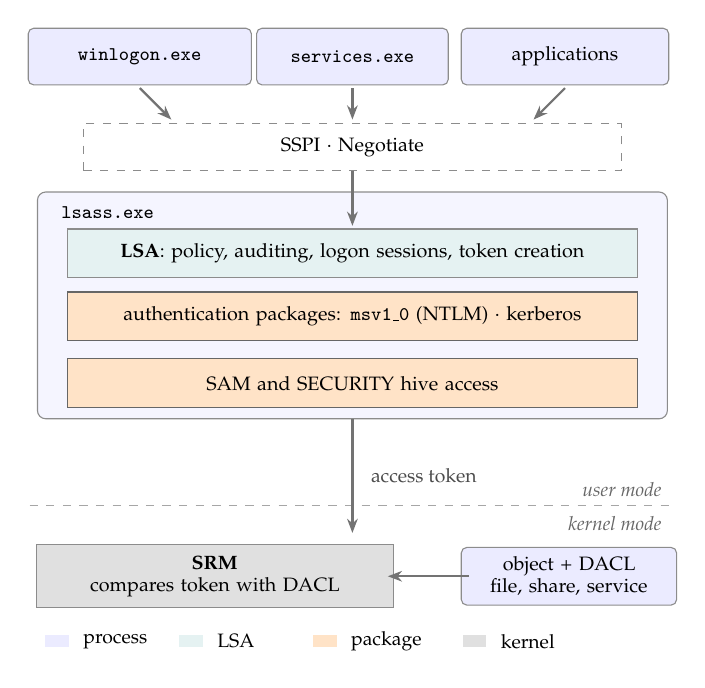
\begin{tikzpicture}[
  proc/.style={draw=black!45, fill=blue!8, rounded corners=2pt, align=center,
               font=\scriptsize, minimum height=0.72cm},
  api/.style={draw=black!45, fill=white, dashed, align=center, font=\scriptsize,
              minimum height=0.6cm},
  sub/.style={draw=black!45, fill=teal!10, align=center, font=\scriptsize,
              minimum height=0.62cm},
  pkg/.style={draw=black!60, fill=orange!22, align=center, font=\scriptsize,
              minimum height=0.62cm},
  kern/.style={draw=black!45, fill=black!12, align=center, font=\scriptsize,
               minimum height=0.8cm},
  arr/.style={-{Stealth[length=1.8mm]}, draw=black!55, thick}
]

% callers -----------------------------------------------------------
\node[proc, text width=2.6cm] (w) at (1.5,0) {\texttt{winlogon.exe}};
\node[proc, text width=2.2cm] (s) at (4.2,0) {\texttt{services.exe}};
\node[proc, text width=2.4cm] (a) at (6.9,0) {applications};

% the interface every caller uses -----------------------------------
\node[api, text width=6.6cm] (sspi) at (4.2,-1.15) {SSPI \textperiodcentered{} Negotiate};

\draw[arr] (1.5,-0.4) -- (1.9,-0.8);
\draw[arr] (4.2,-0.4) -- (4.2,-0.8);
\draw[arr] (6.9,-0.4) -- (6.5,-0.8);

% lsass --------------------------------------------------------------
\draw[draw=black!45, fill=blue!4, rounded corners=3pt] (0.2,-1.72) rectangle (8.2,-4.6);
\node[anchor=north west, font=\scriptsize\bfseries] at (0.38,-1.78) {\texttt{lsass.exe}};

\node[sub, text width=7.0cm] (lsa) at (4.2,-2.5)
  {\textbf{LSA}: policy, auditing, logon sessions, token creation};
\node[pkg, text width=7.0cm] (ap) at (4.2,-3.3)
  {authentication packages: \texttt{msv1\_0} (NTLM) \textperiodcentered{} kerberos};
\node[pkg, text width=7.0cm] (store) at (4.2,-4.15)
  {SAM and SECURITY hive access};

\draw[arr] (4.2,-1.45) -- (4.2,-2.15);

% the boundary and the token -----------------------------------------
\draw[dashed, draw=black!35] (0.1,-5.7) -- (8.3,-5.7);
\node[anchor=south east, font=\scriptsize\itshape, text=black!60] at (8.25,-5.72) {user mode};
\node[anchor=north east, font=\scriptsize\itshape, text=black!60] at (8.25,-5.72) {kernel mode};

\draw[arr] (4.2,-4.6) -- (4.2,-6.05)
  node[midway, right=3pt, font=\scriptsize, text=black!70] {access token};

% authorisation ------------------------------------------------------
\node[kern, text width=4.3cm] (srm) at (2.45,-6.6)
  {\textbf{SRM}\\ compares token with DACL};
\node[proc, text width=2.5cm] (obj) at (6.95,-6.6)
  {object + DACL\\{\scriptsize file, share, service}};

\draw[arr] (5.68,-6.6) -- (4.65,-6.6);

% legend -------------------------------------------------------------
\fill[blue!8] (0.3,-7.5) rectangle (0.6,-7.35);
\node[right, font=\scriptsize] at (0.66,-7.425) {process};
\fill[teal!10] (2.0,-7.5) rectangle (2.3,-7.35);
\node[right, font=\scriptsize] at (2.36,-7.425) {LSA};
\fill[orange!22] (3.7,-7.5) rectangle (4.0,-7.35);
\node[right, font=\scriptsize] at (4.06,-7.425) {package};
\fill[black!12] (5.6,-7.5) rectangle (5.9,-7.35);
\node[right, font=\scriptsize] at (5.96,-7.425) {kernel};

\end{tikzpicture}
\caption{Where a logon is decided, and where it is enforced.}
\label{fig:lsa-stack}
\end{figure}


A successful logon produces an access token, and the token is what authority travels in. It
records the user SID, the group SIDs, the privileges held, a logon SID that identifies the logon
session, the logon type, the integrity level and the session ID (Figure~\ref{fig:token}). The
Security Reference Monitor compares that token with the security descriptor of the object being
opened, and it runs in kernel mode, so the check happens where no process can skip it. It does not
consult the credential store, and it does not ask which package authenticated the caller.

% Figure: what an access token carries. Used in section 2.1.
% The last row is the argument: there is no field for the proof.
\begin{figure}[H]
\centering
\footnotesize
\setlength{\fboxsep}{7pt}
\renewcommand{\arraystretch}{1.25}
\fbox{\begin{tabular}{@{}l@{\hspace{1.6em}}l@{}}
\multicolumn{2}{@{}l}{\textbf{access token}}\\
\midrule
user SID    & \texttt{S-1-5-21-\dots-1105}\\
groups      & \texttt{Domain Users \textperiodcentered{} Helpdesk}\\
privileges  & \texttt{SeChangeNotify \textperiodcentered{} SeDebug}\\
logon SID   & \texttt{S-1-5-5-0-481923}\\
logon type  & 3 (network)\\
integrity   & Medium\\
session     & 1\\
\bottomrule
\end{tabular}}
\caption{What a token carries.}
\label{fig:token}
\end{figure}


That split is deliberate, and it is the opposite of a web application. A web server authenticates
you once, hands back a session identifier, and looks the identifier up on every later request.
Steal the identifier and you hold the session, but the server can also kill it. Windows made the
other trade. An access check happens locally, thousands of times a second, and cannot be a
network round trip, certainly not in 1993 when the model was set. So the decision is cached at
logon: identity, groups and privileges are frozen into an object that any process can be checked
against without touching a directory. The cost is that there is no session to revoke. Disabling an
account does not invalidate a token already issued; it keeps working until the session ends.

The argument of this article reduces to that sentence. The token records who you are and what you
may do, and nothing in it records how you proved it. A logon completed with a hash produces the
same SIDs, the same groups and the same privileges as one completed with the password, because the
package tests possession and the question is then closed. There is no field for NTLM, for Kerberos
or for a password. For authorisation, a hash and a password are the same object.

One adjacent technique deserves a name so the boundary is clear. A process can hold an
impersonation token and act as another user for the lifetime of a thread, which is ordinary
service design and also a way to borrow someone's rights after a compromise. It consumes a live
token rather than a key, it depends on what the engagement hands you, and it is not what this
article is about. The token is the result; what follows is about the key that produces it.

\subsection{Where the hash lives}
\label{sec:hash-lives}

Section~\ref{sec:accounts} covered the databases. Between those and the attack sit four other
places a credential turns up, and they are routinely confused with one another
(Table~\ref{tab:copies}).

\begin{table}[H]
\centering
\small
\renewcommand{\arraystretch}{1.25}
\caption{The four places a credential turns up, and what each gives you.}
\label{tab:copies}
\begin{tabularx}{\textwidth}{@{}>{\raggedright\arraybackslash}m{2.7cm}>{\raggedright\arraybackslash}m{5.0cm}>{\raggedright\arraybackslash}m{1.7cm}Y@{}}
\toprule
Element & What it is & Hash? & What it gives you \\
\midrule
\rowcolor{gray!7} LSASS & the process that runs logons and keeps live session secrets & yes &
  the NT hash of every account with a session open \\
\addlinespace[3pt]
Cached domain credentials & offline verifier used when the domain controller is unreachable & no &
  a salted, iterated verifier: crackable, not replayable \\
\addlinespace[3pt]
\rowcolor{gray!7} WDigest & legacy package that cached the password for single sign-on & plaintext &
  the password itself, if a policy re-enables it \\
\addlinespace[3pt]
Credential Manager & the user's saved-credential vault & no &
  saved passwords, once DPAPI is unlocked \\
\bottomrule
\end{tabularx}
\end{table}

LSASS keeps a hash per live session, so the dump is worth taking on a host where an administrator
has signed in and worth nothing after a reboot. Reading it takes one of three things:

\begin{itemize}[leftmargin=1.6em]
  \item administrator or SYSTEM rights with debug privilege enabled;
  \item a kernel-mode driver;
  \item a dump produced by something that already holds those rights.
\end{itemize}

Cached domain credentials exist so a laptop can log on when the domain controller is unreachable.
The stored value is the password salted with the account name and iterated many times, which makes
it slow to crack and impossible to use as a key. It cannot key an NTLM response, and a tool that
reports cached credentials has found a verifier.

WDigest answered servers that asked for the password rather than a hash, so it kept one. Retention
is off by default from Windows~8.1 and Server~2012~R2, and one legacy policy value turns it back on
for every host that applies the policy. Where it is on, you take the password and derive whatever
else you need.

DPAPI, the Data Protection API, is what applications call instead of writing their own crypto:
they hand it a secret, and it returns ciphertext bound either to the current user or to the machine.
A user-scope key is derived from that user's password, so the ciphertext is tied to the account
rather than to the file it sits in, and LSASS has to unlock the master key at logon before an application
can read its own secrets back.

Credential Manager keeps its entries as DPAPI blobs, each secret encrypted with that profile's
master key and readable only by asking DPAPI to decrypt it. That makes the vault reversible by
design, which is the point: an RDP client has to replay the password, so Windows encrypts it instead
of hashing it. For the credential types Windows writes itself, the blob is the password, so the
decrypt returns plaintext. With the user signed in, LSASS holds the master key unlocked and the
vault opens.

In a default build only the LSASS copy is a key for this attack. WDigest, where a policy has
restored it, is better than one. The other two are what people mistake for it.

\subsection{From password to key material}
\unwritten
% WANT: NT hash = unsalted MD4 over UTF-16LE password, sixteen bytes, no host,
% account or time component. LM as the older sibling in the same record.
% ACADEMIA: why an unsalted fast hash is correct for logon and fatal for reuse.

\subsection{The derivation tree}
\unwritten
% WANT: one figure. password -> NT hash -> NTLM response; password (+ NT hash)
% -> RC4 Kerberos key; password -> AES keys via salted PBKDF2, which the hash
% cannot reach. This asymmetry bounds the whole article.
% FIGURE: fig-hash-derivation (does not exist yet).

\subsection{NTLM in three messages}
\unwritten
% WANT: NEGOTIATE / CHALLENGE / AUTHENTICATE. The server never receives the
% hash; it verifies a response over a challenge it chose (itself, or via the
% DC for a domain account). Then NTLMv1 (deterministic DES) vs NTLMv2.
% FIGURE: fig-ntlm-flow (does not exist yet).

\subsection{Why a captured NTLMv2 is not a hash}
\unwritten
% WANT: NetNTLMv2 is the challenge plus the response. It is a cracking
% candidate, not a key: the response key is bound to user+domain and the proof
% is bound to that server challenge. Most confusion in this area starts here.

\subsection{AD Kerberos in four messages}
\unwritten
% WANT: AS-REQ / AS-REP / TGS-REQ / TGS-REP, the PAC, and pre-auth as an
% encrypted timestamp. Four legs, four different keys.
% ACADEMIA: one figure naming which key protects which leg.
% FIGURE: fig-kerberos-flow (exists).

\subsection{Encryption types: the hinge of everything}
\unwritten
% WANT: for RC4-HMAC the long-term key *is* the NT hash; for AES128/256 it is
% derived from the plaintext. One paragraph, because this single fact decides
% whether pass-the-key works.

\subsection{Carriers: one auth layer, many transports}
\unwritten
% WANT: SMB, MSRPC, WMI/DCOM, WinRM, RDP, LDAP, MSSQL all borrow SSPI/SPNEGO.
% (Table intent: protocol, default mech, NTLM accepted, can it be restricted.)
% Blocking a port relocates the path; it does not remove the capability.

\subsection{Logon types: what gets left behind}
\unwritten
% WANT: type 2/9/10 make the authenticating host retain material; type 3 does
% not. This is the difference between a stepping stone and a dead end, and it
% drives the log story in chapters 7 and 8.

% ======================================================================
% 3. FRAMING  (budget: 1.5 pages)
% Job of the chapter: give the reader one mental model that makes PtH, PtK
% (and the two out-of-scope variants) the same shape, then pin down exactly
% what an attacker must already own.
% ======================================================================
\section{Credential Material as a Bearer Capability}
\label{sec:framing}

\subsection{The unifying property}
% CLAIM (0.4): the authenticator is any secret from which the protocol's
% proof can be computed -- not the password.
% Beats: enumerate what Windows may hold (NT hash, AES keys, ticket session
% keys, PKINIT certificates); each material has a matching "pass-the-X";
% all of them die to the same class of defence (material must not exist on
% the host, or must be unusable off it).

\subsection{Threat model and preconditions}
\subsubsection{Attacker starting positions}
% CLAIM (0.3): two entry points only -- local admin on one host, or material
% obtained out of band. Everything else in the paper follows from these.
\subsubsection{The four preconditions}
% CLAIM (0.4): hash + a service that accepts NTLM + authorisation on the
% target + reachability. Removing any one of them ends the attack, which is
% what chapter 9 exploits.
\subsubsection{Lateral movement, not privilege escalation}
% CLAIM (0.3): PtH transports an existing privilege set; it does not create
% one. Include the local-account caveat: UAC remote restrictions and
% LocalAccountTokenFilterPolicy, the most common reason a real-world attempt
% fails at the last step.

\subsection{Taxonomy and position of this study}
% CLAIM (0.3): a small table positioning PtH, PtK, and the two excluded
% variants by material consumed and protocol family spoken. One paragraph on
% why the excluded two need a different lab (ticket lifecycle, AD CS).

% ======================================================================
% 4. PASS-THE-HASH IN DEPTH  (budget: 3.5 pages)
% Job of the chapter: the reader can reproduce the response computation on
% paper, knows why the wire evidence looks innocent, and knows which
% protocol choice changes the outcome.
% ======================================================================
\section{Pass-the-Hash in Depth}
\label{sec:pth}

\subsection{What the attacker actually holds}
% CLAIM (0.4): sixteen bytes, and their limits.
% Beats: no salt, no key history, no plaintext; where it comes from in
% practice (LSASS, SAM/SECURITY from a backup or shadow copy, a DC dump);
% what it does NOT buy (plaintext, AES Kerberos keys, reuse elsewhere).

\subsection{Computing a valid response without the password}
\subsubsection{The derivation, step by step}
% CLAIM (0.5): the response is HMAC-MD5 keyed with the NT hash over server
% challenge || client challenge || timestamp || target info. Walk it once,
% explicitly, and stop -- the rest of the section is consequences.
\subsubsection{Why this is not replay}
% CLAIM (0.3): fresh timestamp and client challenge per attempt, and the
% binding to the server's challenge, mean a captured response cannot be
% reused against another host. The proof lives in how the bytes were
% produced, not in the bytes.
\subsubsection{Two ways to pass it}
% CLAIM (0.3): speak the protocol from the attacker's host (network logon),
% or write the hash into LSASS and let Windows do it. Different logon types,
% different forensic footprints -- feeds chapters 7 and 8.
% Figure: fig-locality -- what crosses the wire vs what never does.

\subsection{Consequences for signing and sealing}
% CLAIM (0.5): the session key derives from the same hash, so an attacker
% holding the hash can also sign and seal. SMB signing therefore defeats
% relay, not PtH. This is the single most frequently botched claim in
% student write-ups; make it with the derivation, not with an assertion.

\subsection{Protocol coverage}
\subsubsection{SMB}
% CLAIM (0.2): named pipes, ADMIN$/IPC$, service creation or scheduled task;
% what privilege the account needs and what the target records.
\subsubsection{WinRM}
% CLAIM (0.2): no share dependency; often permitted by firewall policy where
% SMB is blocked. Frequently the more reliable path in hardened estates.
\subsubsection{WMI and DCOM}
% CLAIM (0.2): RPC over 135 plus a dynamic range; no file share required.
\subsubsection{RDP with Restricted Admin}
% CLAIM (0.2): a special case worth its own paragraph -- the logon is
% network-type and the hash never reaches the target, it is consumed locally.
\subsubsection{Secondary carriers}
% CLAIM (0.2): MSSQL, LDAP, HTTP/Negotiate. Short; the point is that the
% technique is protocol-agnostic and therefore cannot be fixed per-protocol.

\subsection{Tooling landscape}
% CLAIM (0.4): a table mapping capability to protocol, not a tool review.
% Note our position: orchestrate maintained implementations, own the glue and
% the evidence pipeline. No reimplementation of crypto primitives.

% ======================================================================
% 5. PASS-THE-KEY / OVERPASS-THE-HASH  (budget: 2 pages)
% Gate: only expand past skeleton if the 20 Dec decision is "in".
% ======================================================================
\section{Pass-the-Key: the Kerberos Face of the Same Primitive}
\label{sec:ptk}

\subsection{Why the NT hash is also a Kerberos key}
% TODO
% - RC4-HMAC in AD uses the NT hash directly as the key.
% - AES128/AES256 keys are derived from the plaintext with PBKDF2-like
%   string-to-key salt (realm + username), so they are NOT derivable from the
%   hash. This asymmetry is why RC4 is still negotiated in real estates and
%   why its removal matters.
% - Consequence: an attacker with a hash can request a TGT, and everything
%   downstream is normal Kerberos.

\subsection{Building an AS-REQ from a key}
% TODO
% - Pre-authentication: encrypted timestamp keyed with the client key.
% - What changes when you hold the key instead of the password: nothing,
%   except that you cannot derive AES keys.
% - Result: a TGT whose PAC says the user; then normal TGS requests.
% - Note the downgrade angle: forcing etype 0x17 makes the hash sufficient.

\subsection{What PtK buys over PtH}
% TODO
% - Kerberos-only environments (NTLM disabled) stop PtH but not PtK.
% - Access to services that refuse NTLM.
% - Tickets can be used from non-Windows hosts, so the attacker's OS is irrelevant.

% ======================================================================
% 6. PROOF OF CONCEPT  (budget: 3.0 pages)
% Job of the chapter: justify design decisions and point at the repository
% for mechanics. Declarative how-to lives in poc/README.md; do not duplicate.
% Reader should be able to rebuild the lab from the repo alone.
% ======================================================================
\section{Proof-of-Concept: Environment and Implementation}
\label{sec:poc}

\subsection{Lab topology and isolation}
% CLAIM (0.4): three hosts on a host-only network, no bridged adapter, no
% NAT during execution; snapshot policy yields reproducibility.
% Figure: fig-lab-topology.

\subsection{Identity and permission design}
% CLAIM (0.3): two accounts -- an unprivileged user to prove the limits, and
% a "helpdesk admin" whose rights exist on the client and nowhere else. The
% deliberate misconfiguration under test is stated as such, not hidden.

\subsection{Acquiring the material}
% CLAIM (0.4): local admin on the client reads the credential store; we show
% the hash and never the password, and the account's password is used
% nowhere in the attack. Say plainly that obtaining local admin is the
% expensive part of a real intrusion -- this is the honesty the chapter needs.

\subsection{Scenario A --- PtH over SMB}
% CLAIM (0.5): full sequence, expected artefacts on client and DC, and the
% three ways it can fail (share permissions, token filtering, signing policy).

\subsection{Scenario B --- PtH over WinRM}
% CLAIM (0.3): why it succeeds where SMB is hardened, and what the logs show.

\subsection{Scenario C --- PtK to a TGT}
% CLAIM (0.4): same sixteen bytes, Kerberos client, TGT obtained, service
% ticket used. Delete this subsection entirely if the gate closes.

\subsection{Evidence collection}
% CLAIM (0.4): what we captured and why -- DC and client Security logs, NTLM
% auditing, capture at the client NIC, terminal transcripts; single NTP
% source so events interleave; naming convention the Results chapter cites.

\subsection{Implementation and tooling}
% CLAIM (0.3): we do not reimplement NTLM or Kerberos. Original code is glue:
% environment bootstrap, scenario driver, .evtx extraction that renders the
% chapter 7 tables. Two sentences of justification, then point to the repo.
% No shell listings in the PDF except where the output is the evidence.

% ======================================================================
% 7. RESULTS  (budget: 1.5 pages, mostly tables and figures)
% Rule: every claim here traces to a named file in poc/evidence/.
% Negative results are mandatory -- see 7.3.
% ======================================================================
\section{Results}
\label{sec:results}

\subsection{Success matrix}
% CLAIM (0.5): technique works or not per protocol, with a one-word reason.
% Rows: SMB, WinRM, WMI/DCOM, RDP-restricted, LDAP, MSSQL. Columns: PtH, PtK.
% A matrix with failures in it is more credible than an all-green one.

\subsection{Captured evidence}
% CLAIM (0.5): for each scenario, the same event appears on both ends --
% command outcome, target 4624/4672, DC 4776 or 4768/4769, matching capture.
% Present one compact figure per scenario: log excerpt beside capture excerpt
% on a shared timeline.

\subsection{Boundaries observed}
% CLAIM (0.4): the four negative results and their causes: local-account
% token filtering, an account without target privilege, AES-only enforcement
% blocking PtK, and signing where the session key is unavailable.

\subsection{Cost of the chain}
% CLAIM (0.3): count the steps and the privileges each step required, from
% initial foothold to last hop. Frames the synthesis in chapter 10 without
% editorialising.

% ======================================================================
% 8. DETECTION  (budget: 1.5 pages)
% Authority: every event ID mentioned must be confirmed against Microsoft docs.
% ======================================================================
\section{Detection}
\label{sec:detection}

\subsection{Host telemetry that matters}
% TODO
% - 4624 logon type 3/9 with NTLM as the authentication package, and the
%   detail fields worth alerting on (workstation name vs source IP mismatch,
%   logon without a preceding interactive session).
% - 4672 special privileges assigned, following a type-3 logon.
% - 4776 credential validation on the DC and how it differs from 4624.
% - 4768/4769 for the PtK side, including cipher/etype fields.
% - 4648 explicit credential use as a baseline comparator.

\subsection{What the attack cannot hide}
% TODO
% - The target always logs a successful network logon; the DC always validates.
%   The attacker controls neither. This is the structural weakness of PtH.
% - Therefore detection is about baselining "who logs on where with NTLM",
%   not about catching a signature.

\subsection{Network-level signals}
% TODO
% - NTLMSSP in clear where the carrier is not encrypted; Negotiate downgrade.
% - NTLM auditing on the DC as the cheapest visibility win.

\subsection{Behavioural and deception controls}
% TODO
% - Honeytoken accounts / canary credentials in LSASS; any use is high signal.
% - Baseline deviation: NTLM logon to a server that normally only does Kerberos.
% - Short paragraph on EDR: what a memory read of LSASS looks like.

% ======================================================================
% 9. EFFECTS AND MITIGATION  (budget: 2 pages)
% Structure: damage -> controls by layer -> measured effect in our lab.
% Every control gets: what it stops, what it costs, what it does NOT stop.
% ======================================================================
\section{Effects and Mitigation}
\label{sec:mitigation}

\subsection{Damage model}
% TODO
% - PtH converts one compromised workstation into the privileges of every
%   privileged account that touched it. Quantify: one host, N cached admins.
% - The compounding effect over time: each hop adds hashes.
% - Historical anchors: NotPetya and similar campaigns as the reference case.

\subsection{Credential protection}
% TODO
% - Credential Guard / LSA protection (PPL): stops remote extraction of the
%   hash; explicitly state what it does not do (a local admin can still
%   abuse a live session).
% - Protected Users group and its consequences (no NTLM, no delegation, no
%   RC4) -- and the operational pain it causes.
% - Disable WDigest; restrict cached credentials.

\subsection{Protocol hardening}
% TODO
% - Disable or restrict NTLM (audit first, then block per service); this is
%   the only control that removes the PtH path outright.
% - Kerberos: remove RC4, require AES, enforce FAST/armoring -- this removes
%   the PtK path.
% - SMB signing and encryption: state precisely that they address relay and
%   tampering, not hash possession.
% - EPA / channel binding for the HTTP-facing cases.

\subsection{Architectural controls}
% TODO
% - Tiered administration, PAW, LAPS for local accounts, JIT elevation,
%   gMSA/service accounts. Frame as "reduce how many hashes are reachable
%   from a workstation", not as a checklist.

\subsection{Measured effectiveness in the lab}
% TODO -- the strongest section of the essay
% - Table: control applied -> scenario A/B/C outcome -> cost/limitation.
% - Include one control that did not help, and explain why. That single
%   negative result demonstrates understanding.
% Figure: fig-mitigation-matrix.

% ======================================================================
% 10. SYNTHESIS  (budget: 1.0 page)
% Job of the chapter: answer the question the title implies -- so when does
% this still work? A decision chain, not a summary of the paper.
% ======================================================================
\section{When These Attacks Actually Work}
\label{sec:synthesis}

\subsection{The precondition chain as a decision procedure}
% CLAIM (0.4): five questions in order, each one able to end the attack:
%   1. Is NTLM accepted anywhere on the path?        -> PtH viable
%   2. Is RC4 enabled for the account?               -> PtK viable
%   3. Is the hash reachable on a host we already own? -> both viable
%   4. Is extraction blocked (Credential Guard/PPL)? -> extraction dead, live
%                                                       session reuse is not
%   5. Is the account authorised on the target?      -> the real bottleneck
% Most real intrusions die at 5, and almost nobody writes that down.

\subsection{Where it fails in a modern estate}
% CLAIM (0.3): concrete failure modes we observed plus the ones we can argue
% from the protocol: token filtering, NTLM disabled per service, AES-only,
% Protected Users, tiered admin with no overlapping local admins.

\subsection{What survives the deprecation}
% CLAIM (0.3): NTLM deprecation and RC4 removal shrink this space over the
% next few years, but the class of attack survives as long as any protocol
% authenticates on derived key material -- which is exactly why ticket and
% certificate abuse are the same argument in different clothes.

% ======================================================================
% 11. CONCLUSION  (budget: 0.5 page -- no subsections, by design)
% Three moves only: the finding, what the PoC showed (numbers), the control
% worth funding first plus the honest residual risk. No new material.
% ======================================================================
\section{Conclusion}
\label{sec:conclusion}

% CLAIM: the protocol is not broken, the key handling is; therefore the fix is
% to stop the key from existing on hosts we do not control, not to strengthen
% the cipher. Close on the residual risk: as long as an authenticated session
% can be replayed or a key can be recomputed, no protocol hardening finishes
% the job.


\printbibliography[heading=bibintoc,title={References}]

\appendix
% ======================================================================
% APPENDIX  (no page budget -- as long as the evidence needs)
% Rule: nothing here is prose. Reference poc/ for the authoritative version.
% ======================================================================
\section{Lab Build}
% VM specs, OS build numbers, roles installed, network configuration,
% snapshot names. Summarised from poc/lab/, not duplicated.

\section{Full Log Excerpts}
% The untruncated event behind every row of the chapter 7 tables, one block
% per scenario, with the exact event ID and the fields we relied on.

\section{Capture Index}
% Table: file name, host, capture filter, what to look at. Binaries stay in
% the repository release, not in git history.

\section{Tool and Version Inventory}
% Every tool used, version string, and the exact commit or release tag.
% Required for the reproducibility claim in chapter 6.


\end{document}
